\chapter{渐进理论初步}

\begin{theorem}[Scheffe Theorem]
	设$\{f_n\}$是测度空间$(X,\mathscr{F},\mu)$上的可积函数列,$f$是$(X,\mathscr{F},\mu)$上的可积函数,$f_n\overset{a.e.}{\longrightarrow}f$,则
\end{theorem}
\begin{theorem}[Slutsky Theorem]\label{theo:Slutsky}
	设$\{f_n\}$和$\{g_n\}$是概率空间$(X,\mathscr{F},P)$上的随机变量序列,$f$是$(X,\mathscr{F},P)$上的随机变量,$c\in\mathbb{R}^{}$。若:
	\begin{equation*}
		f_n\overset{L}{\longrightarrow}f,\quad g_n\overset{P}{\longrightarrow}c
	\end{equation*}
	则:
	\begin{enumerate}
		\item $f_n+g_n\overset{L}{\longrightarrow}f+c$;
		\item $g_nf_n\overset{L}{\longrightarrow}cf$;
		\item 当$c\ne0$时,$\dfrac{f_n}{g_n}\overset{L}{\longrightarrow}\dfrac{f}{c}$。
	\end{enumerate}
\end{theorem}
\begin{proof}
	
\end{proof}
\begin{theorem}
	设$\{\mathbf{X_n}\}$是概率空间$(X,\mathscr{F},P)$上的$p$维随机向量序列,$X$是$(X,\mathscr{F},P)$上的$p$维随机向量,$g$是$(\mathbb{R}^{p},\mathcal{B}^p)$到$(\mathbb{R}^{q},\mathcal{B}^q)$上的可测函数,且$g\;$a.s连续于,则:
	\begin{enumerate}
		\item $\mathbf{X_n}\overset{a.s.}{\longrightarrow}X\Rightarrow g(\mathbf{X_n})\overset{a.s.}{\longrightarrow}g(X)$;
		\item $\mathbf{X_n}\overset{P}{\longrightarrow}X\Rightarrow g(\mathbf{X_n})\overset{P}{\longrightarrow}g(X)$;
		\item $\mathbf{X_n}\overset{d}{\longrightarrow}X\Rightarrow g(\mathbf{X_n})\overset{d}{\longrightarrow}g(X)$;
	\end{enumerate}
\end{theorem}
\begin{proof}
	
\end{proof}


\section{大数定律}

\subsection{弱大数定律}
\begin{definition}
	设$\{X_n\}$是一个随机变量序列,若
	\begin{equation*}
		\frac{1}{n}\sum_{i=1}^{n}X_i\overset{P}{\longrightarrow}\frac{1}{n}\sum_{i=1}^{n}\operatorname{E}(X_i)
	\end{equation*}
	则称$\{X_n\}$服从\gls{WeakLawOfLargeNumbers}。
\end{definition}
\begin{theorem}[Markov's Weak Law of Large Numbers]
	设$\{X_n\}$是一个随机变量序列,若:
	\begin{equation*}
		\lim_{n\to+\infty}\left[\frac{1}{n^2}\operatorname{Var}\left(\sum_{i=1}^{n}X_i\right)\right]=0
	\end{equation*}
	则$\{X_n\}$服从弱大数定律。
\end{theorem}
\begin{proof}
	由\cref{ineq:Chebyshev}可知对任意的$\varepsilon>0$有:
	\begin{equation*}
		P\left(\left|\frac{1}{n}\sum_{i=1}^{n}X_i-\frac{1}{n}\sum_{i=1}^{n}\operatorname{E}(X_i)\right|\geqslant\varepsilon\right)\leqslant\frac{\operatorname{Var}\left(\dfrac{1}{n}\sum\limits_{i=1}^{n}X_i\right)}{\varepsilon^2}=\frac{1}{n^2\varepsilon^2}\operatorname{Var}\left(\sum_{i=1}^{n}X_i\right)\to0\qedhere
	\end{equation*}
\end{proof}
\begin{corollary}
	由Markov's Weak Law of Large Numbers可以推出:
	\begin{enumerate}
		\item (Chebyshev's Weak Law of Large Numbers)设$\{X_n\}$为一列互不相关的随机变量,若对于任意的$n\in\mathbb{N}^+$,有$\operatorname{Var}(X_i)\leqslant c<+\infty$,则$\{X_n\}$服从弱大数定律。
		\item (Bernoulli's Weak Law of Large Numbers)设$\{X_n\}$为一列独立同两点分布$b(1,p)$的随机变量,则$\{X_n\}$服从弱大数定律。
	\end{enumerate}
\end{corollary}
\begin{proof}
	(1)因为$\{X_n\}$互不相关,所以\info{以后写不相关的和的方差,需要注意从乘积期望开始写,还得链接方差线性变换的性质}:
	\begin{equation*}
		\operatorname{Var}\left(\frac{1}{n}\sum_{i=1}^{n}X_i\right)=\frac{1}{n^2}\sum_{i=1}^{n}\operatorname{Var}(X_i)\leqslant\frac{1}{n^2}nc=\frac{c}{n}\to0
	\end{equation*}\par
	(2)由两点分布的性质或者(1)直接可得。
\end{proof}
%\begin{theorem}[khinchin's Weak Law of Large Numbers]\label{theo:WeakLawOfLargeNumbers}
%%	设$\{Xm_n\}$是一列独立同分布的随机变量,若$X_n$的数学期望有限,则$\{X_n\}$服从大数定律。
%\end{theorem}
\begin{proof}
	\info{需要写完特征函数}
\end{proof}

\begin{theorem}[Strong Law of Large Numbers]
	\label{theo:StrongLawOfLargeNumbers}
	设$\{X_n\}$为一列独立同分布的随机变量,服从的分布的均值为$\mu$且满足$\operatorname{E}(|X_i|)<+\infty$,则有:
	\begin{equation*}
		P\left(\lim_{n\to+\infty}\bar{X}_n\ne\mu\right)=0
	\end{equation*}
	即$\bar{X}_n\overset{\text{a.e.}}{\longrightarrow}\mu$。
\end{theorem}

\section{连续性校正}

\subsection{使用原因}
由中心极限定理,独立同分布的随机变量序列$X_i,\;i=1,2\dots,n$的和$\sum\limits_{i=1}^{n}X_i$将在随机变量个数$n\to+\infty$时服从正态分布,因此,在某些情况下,我们可以利用正态分布CDF(Cumulative Distribution Function)值来近似一些难以计算的离散型随机变量(Discrete Variable)的CDF值。

\begin{figure}[htbp] 
	\centering 
	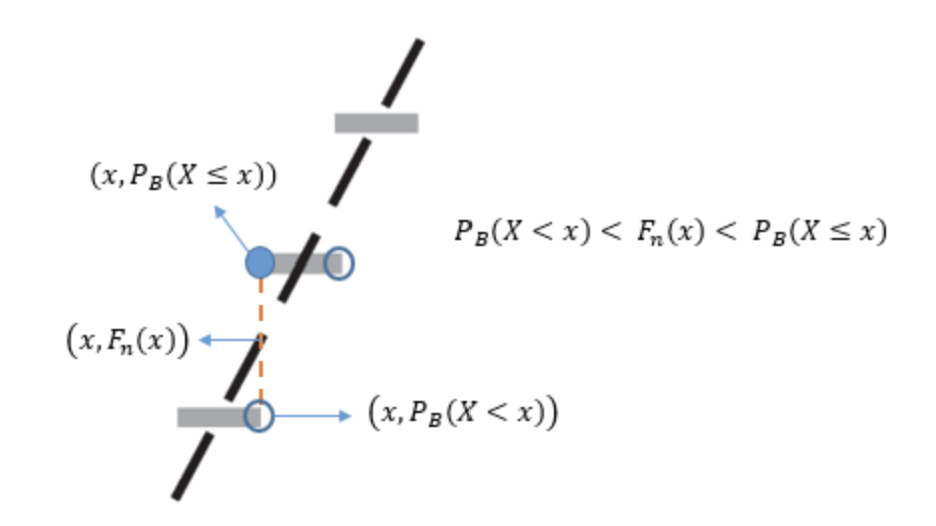
\includegraphics{probability-theory/chapter4/CDF-of-c-and-d-variables.png} 
	\caption{连续型、离散型随机变量CDF图} 
\end{figure}

\hspace{2em}对于离散型随机变量,常出现$P(X<x)\ne P(X\leqslant x)$,而对于连续型随机变量(Continuous Variable),二者的值是相等的,因此,CDF值的近似将出现以下问题:
\begin{enumerate}
	\item 使用正态分布CDF值近似$P(X\leqslant x)$时近似值偏小。
	\item 使用正态分布CDF值近似$P(X< x)$时近似值偏大。
\end{enumerate}
\hspace{2em}而我们会想要得到一个一致的近似,即对于以上两个近似,结果总是一致地偏大或偏小,这样利于分析。

\subsection{具体方法}
\begin{itemize}
	\item 根据近似的分布选择一个$\alpha\in (-1,1)$,一般选择$\pm\frac{1}{2}$。
	\item 使用正态分布CDF值$F(\frac{x+\alpha-\mu}{\sigma})$近似$P(X< x)$与$P(X\leqslant x)$。
\end{itemize}